% Created 2021-01-21
% Intended LaTeX compiler: pdflatex
\documentclass[11pt]{article}
\usepackage[utf8]{inputenc}
\usepackage[T1]{fontenc}
\usepackage{graphicx}
\usepackage{grffile}
\usepackage{longtable}
\usepackage{wrapfig}
\usepackage{rotating}
\usepackage[normalem]{ulem}
\usepackage{amsmath}
\usepackage{textcomp}
\usepackage{amssymb}
\usepackage{amsthm}
\usepackage{capt-of}
\usepackage{hyperref}
\usepackage{algorithm}
\usepackage[noend]{algpseudocode}
\usepackage{algorithmicx}
\usepackage{courier} %% Sets font for listing as Courier.
\usepackage{listings, xcolor}
\usepackage[shortlabels]{enumitem}
\author{Mingzhe Wang\\wangm235@mcmaster.ca
\and Xing Li\\li64@mcmaster.ca}
\date{\today}
\title{Assignment 3}

% table display
\renewcommand{\arraystretch}{1.3}

% algpseudocode modifications
\newcommand*{\Let}[2]{\State #1 $\gets$ \parbox[t]{\linegoal}{#2\strut}}
\algnewcommand\algorithmicinput{\textbf{INPUT: }}
\algnewcommand\Input{\item[\algorithmicinput]}
\algnewcommand\algorithmicoutput{\textbf{OUTPUT: }}
\algnewcommand\Output{\item[\algorithmicoutput]}

% algorithmic modifications
\makeatletter
\newcommand{\ALOOP}[1]{\ALC@it\algorithmicloop\ #1%
  \begin{ALC@loop}}
\newcommand{\ENDALOOP}{\end{ALC@loop}\ALC@it\algorithmicendloop}
\renewcommand{\algorithmicrequire}{\textbf{Input:}}
\renewcommand{\algorithmicensure}{\textbf{Output:}}
\newcommand{\algorithmicbreak}{\textbf{break}}
\newcommand{\BREAK}{\STATE \algorithmicbreak}
\makeatother

\begin{document}
\maketitle
\tableofcontents

\newpage

\section{Question 1}
For Prim's Algorithm, we need to run Prim's Algorithm for each unmarked vertex to find minimum spanning forest. That is, we split the prim function from the PrimMST constructor and then add a loop to cover all unmarked vertex. The implementation is listed below, as compared to original Prim's MST algorithm in textbook page 622.\\
\begin{lstlisting}
 public PrimMST(EdgeWeightedGraph G) {
        edgeTo = new Edge[G.V()];
        distTo = new double[G.V()];
        marked = new boolean[G.V()];
        pq = new IndexMinPQ<Double>(G.V());
        for (int v = 0; v < G.V(); v++)
            distTo[v] = Double.POSITIVE_INFINITY;

        for (int v = 0; v < G.V(); v++) 
            if (!marked[v]) prim(G, v); 
    }

    private void prim(EdgeWeightedGraph G, int s) {
        distTo[s] = 0.0;
        pq.insert(s, distTo[s]);
        while (!pq.isEmpty()) {
            int v = pq.delMin();
            scan(G, v);
        }
    }
\end{lstlisting}

~\newline\noindent
For Kruskal’s algorithm, we do not need to modify any part. The original algorithm can be used to compute the minimum spanning forest in unconnected graph.

\section{Question 2}
\begin{itemize}
\item If the deleted edge is not on the old MST, then the old MST is the MST of the new graph. (Because the MST is the spanning tree with the least weight of its edges, deleting other edges will not affect the output MST.)
\item Otherwise, the MST will be split to two components. (Because as the spanning tree property, the spanning tree cannot have any cycle). Then we loop through all the edges, and add the minimum weight edge that connects the two components to the old MST, the updated MST will be the MST of the new graph. (By the Cut Property)
\end{itemize}
The above process will take $O(E)$ time, because we loops through all edges once.

\section{Question 3}
The outline is as follow:
\begin{itemize}
\item Add a new vertex s. 
\item Add an edge of length 0 from s to each vertex in S.
\item Run Dijkstra's algorithm, with s being the source vertex.
\item Return the least value in $\{distTo[t], t \in T\}$, where t is an vertex in T.
\end{itemize}

~\newline\noindent
Explanation for $O(E \log V)$:

~\newline\noindent
The first step takes $O(1)$ time, the second step takes $O(V)$ time, the third step takes $O((V+E)\log V)$ time, the fourth step takes $O(V)$ time. It's reasonable to assume $E > V$, then $O((V+E)\log V) = O(E \log V)$ and $E \log V > V \log V > V > 1$. Therefore, the total time complexity will be  $O(E \log V)$.

\section{Question 4}
For all paths from s to other vertices, they can be divided into three categories: 
\begin{enumerate}[a)]
\item not monotonic 
\item strictly increasing
\item strictly decreasing
\end{enumerate}
What we need to do is:
\begin{enumerate}
\item filter out a
\item find the shortest path $p_b$ in b
\item find the shortest path $p_c$ in c
\item choose the minimum in $p_b$ and $p_c$
\end{enumerate}
As there is no specification in the question that all of the weights are positive, we have to assume there could be negative weights. Therefore, we modify Bellman-Ford algorithm as below, and assume there is no negative cycle.

\begin{algorithm}
\caption{Find the monotonic shortest path}
\begin{algorithmic}[1]
\Procedure{getMonotonicShortestPath}{$weightedGraph$, $source$}
\State Initiate a dictionary P 
\State // to keep the dictionaris of last edges for each vertex
\State distTo1, edgeTo1 = getShortestPath(Increasing)
\State distTo2, edgeTo2 = getShortestPath(Decreasing)
\For{vertex v in $weightedGraph$}
\If{distTo1[v] < distTo2[v]}
	\State P[v] = edgeTo1
\Else
	\State P[v] = edgeTo2
\EndIf
\EndFor
\Return P
\\
\Procedure{getShortestPath}{$incOrDec$}
\State Initiate a dictionary $distTo$ 
\State // to keep the shortest distance from $source$ to each vertex
\State Initiate a dictionary $edgeTo$ 
\State // to keep the last edge of the shortest path from $source$ to each vertex
\State initiate a queue Q
\State Initiate a dictionary $onQ$ 
\State // to track whether the vertex is on the queue
\State $distTo$[$source$] = 0, $dist$[$v$] = $\infty$ for other vertices
\State Q.enqueue(source), onQ[$source$] = true
\State $edgeTo$[$source$] = dummy edge
\If{$incOrDec$ = increasing}
	\State $edgeTo$[$source$].weight= - $\infty$
\Else
	\State $edgeTo$[$source$].weight = $\infty$
\EndIf
\While {Q is not empty}
	\State v = Q.dequeue()
	\State onQ[v] = false
	\State relax(v)
\EndWhile
\Return $distTo$, $edgeTo$
\\
\Procedure{relax}{$vertex$}
\For{all adjacent edges $e$ of $vertex$} 
	\State w = e.to
	\State e1 = $edgeTo$[$vertex$]
	\If { ($incOrDec$ = increasing and e.weight > e1.weight) or ($incOrDec$ = decreasing and e.weight < e1.weight)}
	\If {$distTo$[w] > $distTo$[$Vertex$] + e.weight}
		\State $distTo$[w] = $distTo$[$Vertex$] + e.weight
		\State $edgeTo$[w] = e
		\If{not onQ[w]}
			\State Q.enqueue(w)
			\State onQ[w] = true
		\EndIf
	\EndIf
	\EndIf
\EndFor
\EndProcedure

\EndProcedure
\EndProcedure
\end{algorithmic}
\end{algorithm}
\newpage
\section{Question 5}

If we don't need to keep the array stable, we can simply copy the key for the times that it is counted. In this way, we don't need the auxiliary array.
\begin{algorithm}
\caption{Key-indexed counting with constant extra space}
\begin{algorithmic}[1]
\Procedure{keyIndexedCounting}{$array$}
\State // Count frequencies of each letter using key as index
\State Initiate an array $Count$ for counting with default value 0
\For{element in $array$}
	\State $Count[element] \gets Count[element] + 1$ 
\EndFor
\State // Update the original array as per the order in $Count$,
\State // and copy an element for Count[element] times
\State i $\gets$ 0
\State j $\gets$ 0
\While{i < |array|}
	\For{k = 1 to Count[j]}
		\State $array[i] \gets j$
		\State $i \gets i + 1$
	\EndFor
	\State $j \gets j + 1$
\EndWhile
\EndProcedure
\end{algorithmic}
\end{algorithm}

\section{Question 6}
We use KMP algorithm to check whether one string (string2 with length n) is a substring of the concatenation of the other string (string1 + string1, with length 2n), so the time complexity is O(n + 2n) = O (3n).
Based on big O's definition, O(3n) means that there exists constant c > 0 and $n_0 \ge 0 $ such that $ 0 \le T(n) \le c * (3n) $ for all $n \ge n_0$, which is equivalent to the statement that there exists constant $c_1 = 3*c$ > 0 and $n_0 \ge 0 $ such that $ 0 \le T(n) \le c_1 *n) $ for all $n \ge n_0$. Therefore, our algorithm runs in O(n) time.
\begin{algorithm}
\caption{Cyclic rotation}
\begin{algorithmic}[1]
\Procedure{isCyclicRotation}{$string1$, $string2$}
\State string3 $\gets$ Concatenate $string1$ and $string1$
\State \Return KMP1($string3$, $string2$)
\EndProcedure
\Procedure{KMP1}{$word$, $pattern$}
\State //This is a variation of KMP algorithm. It returns true if one pattern match is found.
\State i = 0, j = 0, $B_p$ = getBoarderArray($pattern$)
\While{i < |$word$|}
	\If{pattern[j + 1] = word[i + 1]}
		\State j = j + 1, i = i + 1
	\EndIf
	\If{j = |$pattern$|}
		\Return True
	\Else
		\If{j = 0}
			\State i = i + 1
		\Else
			\State j = $B_p$[j]
		\EndIf
	\EndIf
\EndWhile
\Return False
\EndProcedure
\Procedure{getBoarderArray}{$string$}
\State initiate an array $\beta$
\State $\beta$[1] = 0
\For{i = 1 to |$string$| - 1}
	\State b = $\beta$[i]
	\While{b > 0 and $string$[i + 1] $\neq$ $string$[b + 1]}
		b = $\beta$[b]
	\EndWhile 
	\If{$string$[i + 1] = $string$[b + 1]} 
		\State  $\beta$[i + 1] = b + 1
	\Else
		\State$\beta$[i + 1] = 0
	\EndIf
\EndFor
\Return $\beta$
\EndProcedure
\end{algorithmic}
\end{algorithm}

\newpage

\section{Question 7}
Our algorithm takes three steps:

Step 1. We use KMP algorithm to get all indexes of a match for substring u (length m) in string s (length n). That will be an array of increasing natural numbers.
For example, if u = abcab and s = abcabcababcababcababcab, the array will be [0, 3, 8, 13, 18]. The time complexity is O(n + m). There exists constant $c_1$ > 0 and $n_1 \ge 0 $ such that $ 0 \le T(n) \le c_1 * (n + m) $ for all $n \ge n_1$.

Step 2. After that we will go through the sequence and generate a new array with length n to tag the consecutivity [1, 0, 0, 1, 0, 0, 0, 0, 2, 0, 0, 0, 0, 3, 0, 0, 0, 0, 4, 0, 0, 0, 0]. The time complexity is O(n). There exists constant $c_2$ > 0 and $n_2 \ge 0 $ such that $ 0 \le T(n) \le c_2 * n $ for all $n \ge n_2$.

Step 3. We go through the new array, find the maximum, and returns its index deducted by the product of m and its value minus 1. In our case, it's 18 - 5 * (4 -1) = 3. The time complexity is also O(n). There exists constant $c_3$ > 0 and $n_3 \ge 0 $ such that $ 0 \le T(n) \le c_3 * n $ for all $n \ge n_3$.

Therefore,  there exists constant $c = max(c_1, c_2, c_3)$ > 0 and $n = max(n_1, n_2, n_3) \ge 0 $ such that $ 0 \le T(n) \le c * (m +3n) $ for all $n \ge n_3$. The overall time complexity is O(m + 3n), which is linear.  

\begin{algorithm}
\caption{Get index of the longest Tandem repeat}
\begin{algorithmic}[1]
\Procedure{getIndexOfLongestTandemRepeat}{$u$, $s$}
\State indexList $\gets$ KMP($s$, $u$)
\State Initiate an array c of length $s$ - 1 with default value 0
\State // It is to track the consecutivity
\For{i = 0 to |indexList| - 1}
	\State prevIndex = indexList[i] - |$u$|
	\If{prevIndex $ \ge 0$}
		\State c[indexList[i]] = c[prevIndex] + 1
	\Else
		\State c[indexList[i]] = 1
	\EndIf
\EndFor
\State max, indexOfMax = 0, -1 // -1 means no tandem repeat is found
\For{i = 0 to |c| - 1}
	\If{c[i] > max}
		\State max, indexOfMax = c[i], i
	\EndIf
\EndFor
\Return indexOfMax - |$u$| * (max - 1)
\EndProcedure
\Procedure{KMP}{$word$, $pattern$}
\State i = 0, j = 0, indexList = $\emptyset$, $B_p$ = getBoarderArray($pattern$)
\While{i < |$word$|}
	\If{pattern[j + 1] = word[i + 1]}
		\State j = j + 1, i = i + 1
	\EndIf
	\If{j = |$pattern$|}
		\State indexList = indexList $\cup$ \{i - j + 1\}
		\State j = $B_p$[j]
	\Else
		\If{j = 0}
			\State i = i + 1
		\Else
			\State j = $B_p$[j]
		\EndIf
	\EndIf
\EndWhile
\Return indexList
\EndProcedure
\Procedure{getBoarderArray}{$string$}
\State initiate an array $\beta$
\State $\beta$[1] = 0
\For{i = 1 to |$string$| - 1}
	\State b = $\beta$[i]
	\While{b > 0 and $string$[i + 1] $\neq$ $string$[b + 1]}
		b = $\beta$[b]
	\EndWhile 
	\If{$string$[i + 1] = $string$[b + 1]} 
		\State  $\beta$[i + 1] = b + 1
	\Else
		\State$\beta$[i + 1] = 0
	\EndIf
\EndFor
\Return $\beta$
\EndProcedure
\end{algorithmic}
\end{algorithm}

\newpage
\section{Question 8}
\subsection{Question 8(i)}
\begin{center}
\begin{tabular}{ c c c }
 char & freq & encoding \\ 
 \hline
 h & 21 & 0 \\
 g & 13 & 10 \\  
 f & 8 & 110 \\  
 e & 5 & 1110 \\    
 d & 3 & 11110 \\   
 c & 2 & 111110 \\       
 a & 1 & 1111110 \\    
 b & 1 & 1111111 \\    
\end{tabular}
\end{center}

The process (some steps are omitted):
\begin{figure}[hbt!]
  \centering
  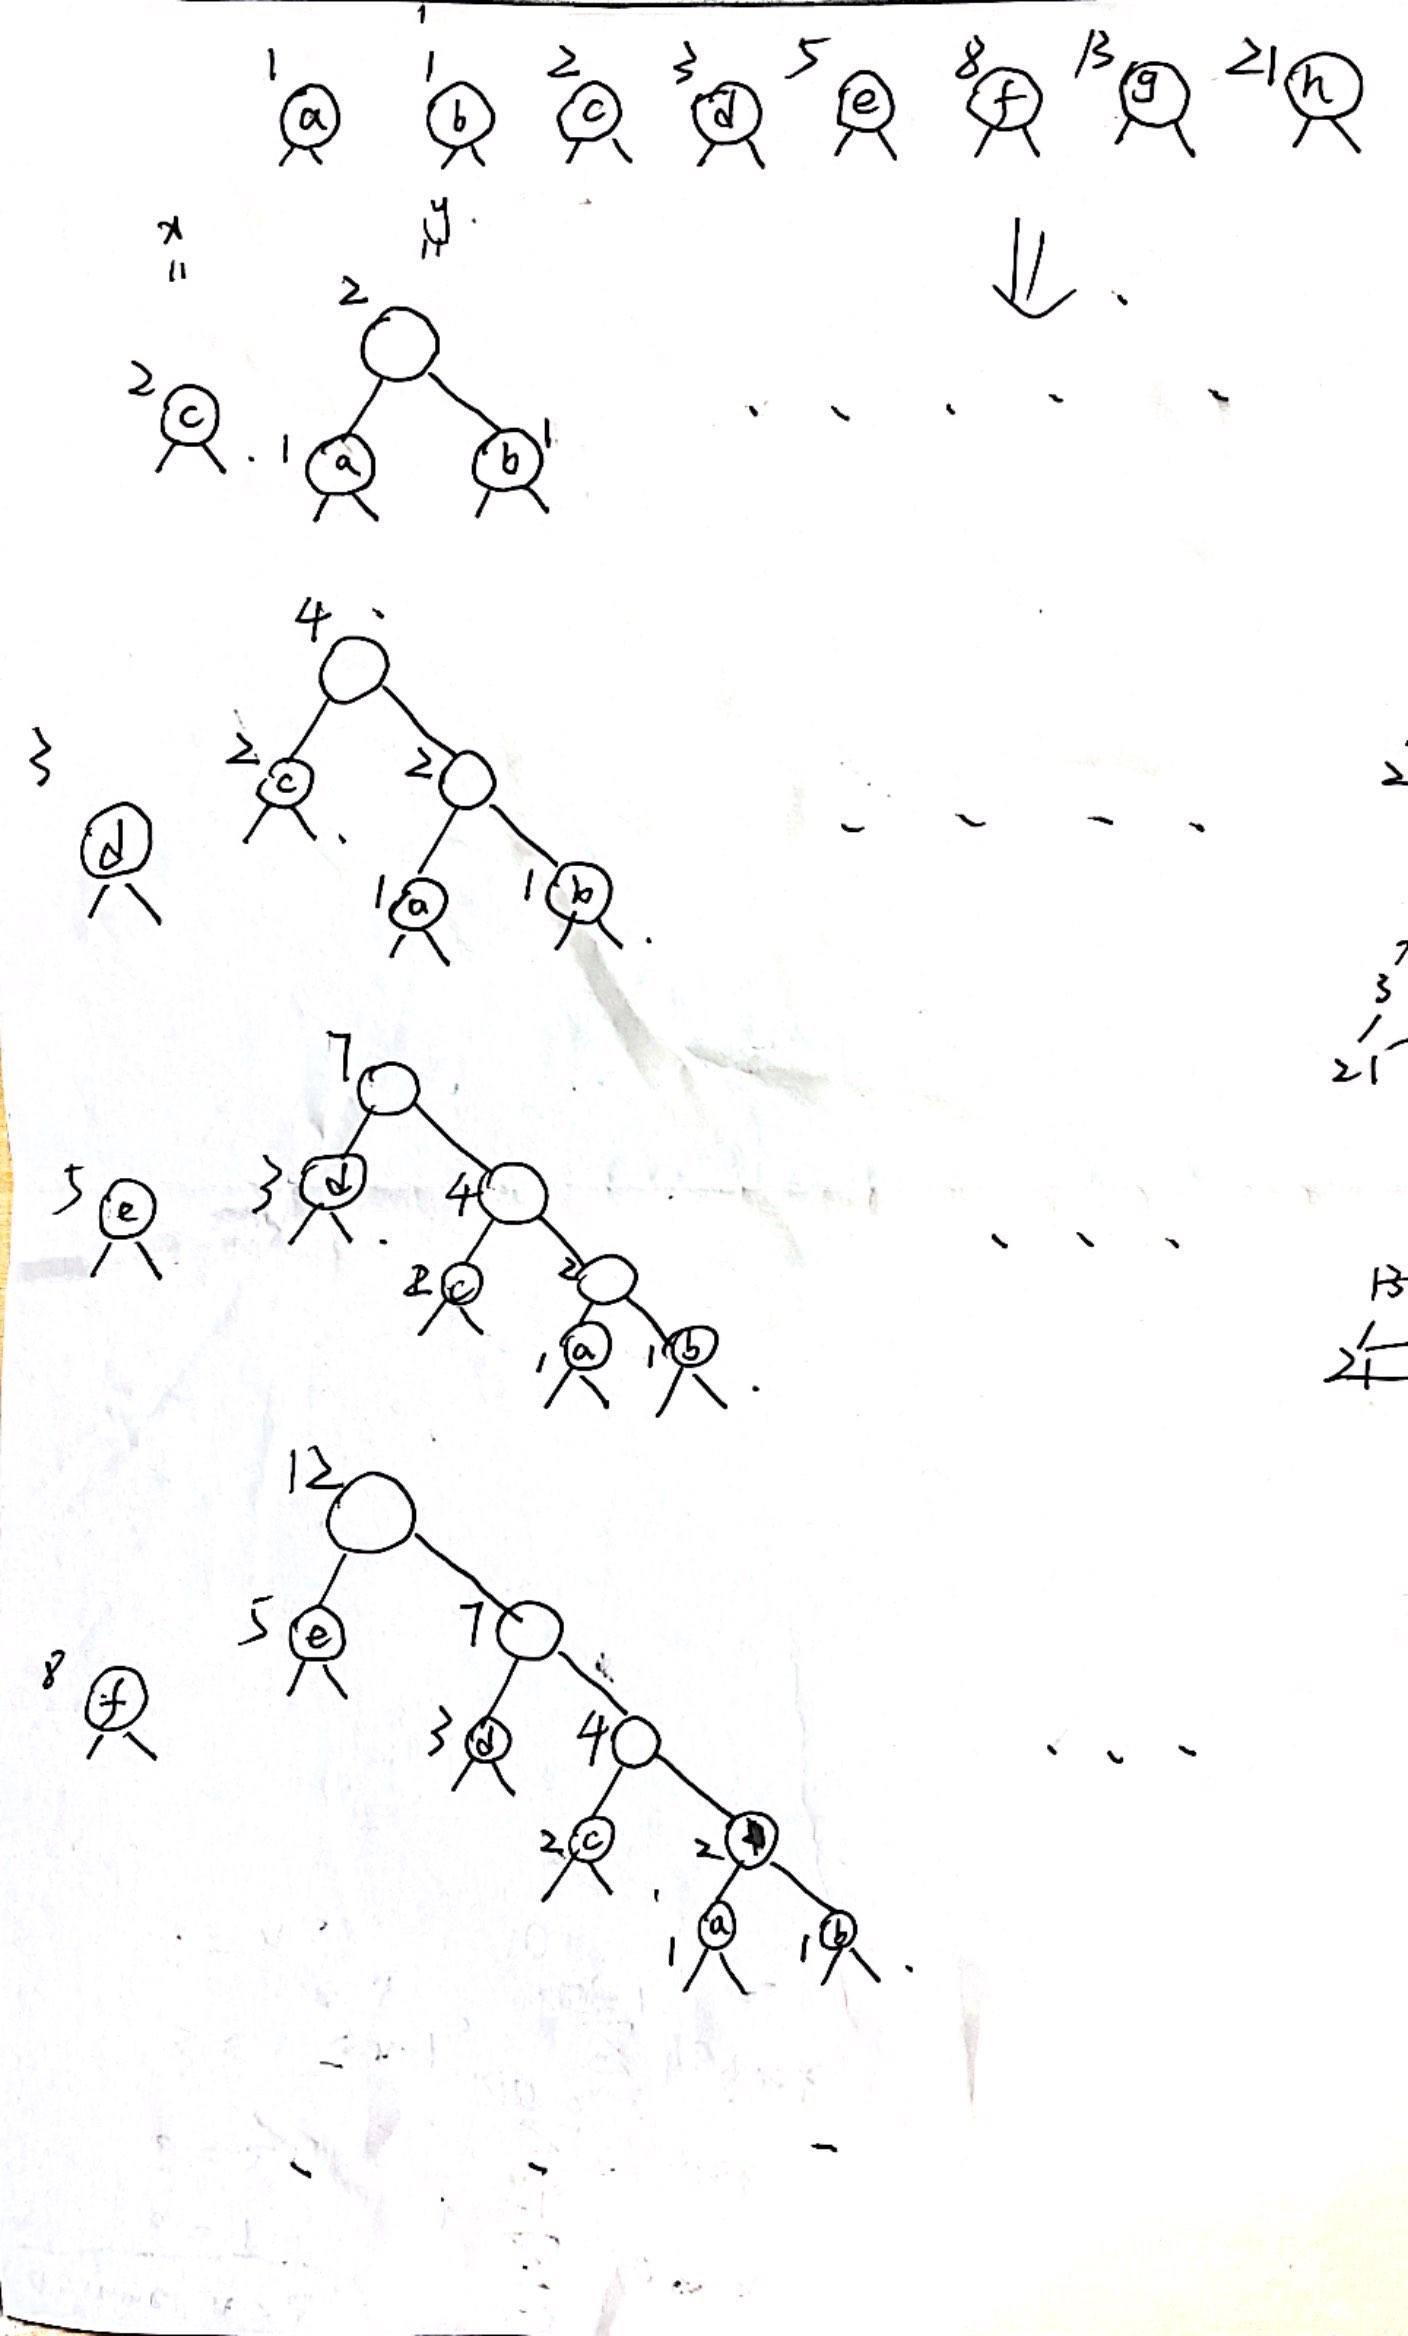
\includegraphics[width=0.5\textwidth]{Huffman_code_process.jpg}
\end{figure}

~\newline\noindent
The result (some steps are omitted):
\begin{figure}[hbt!]
  \centering
  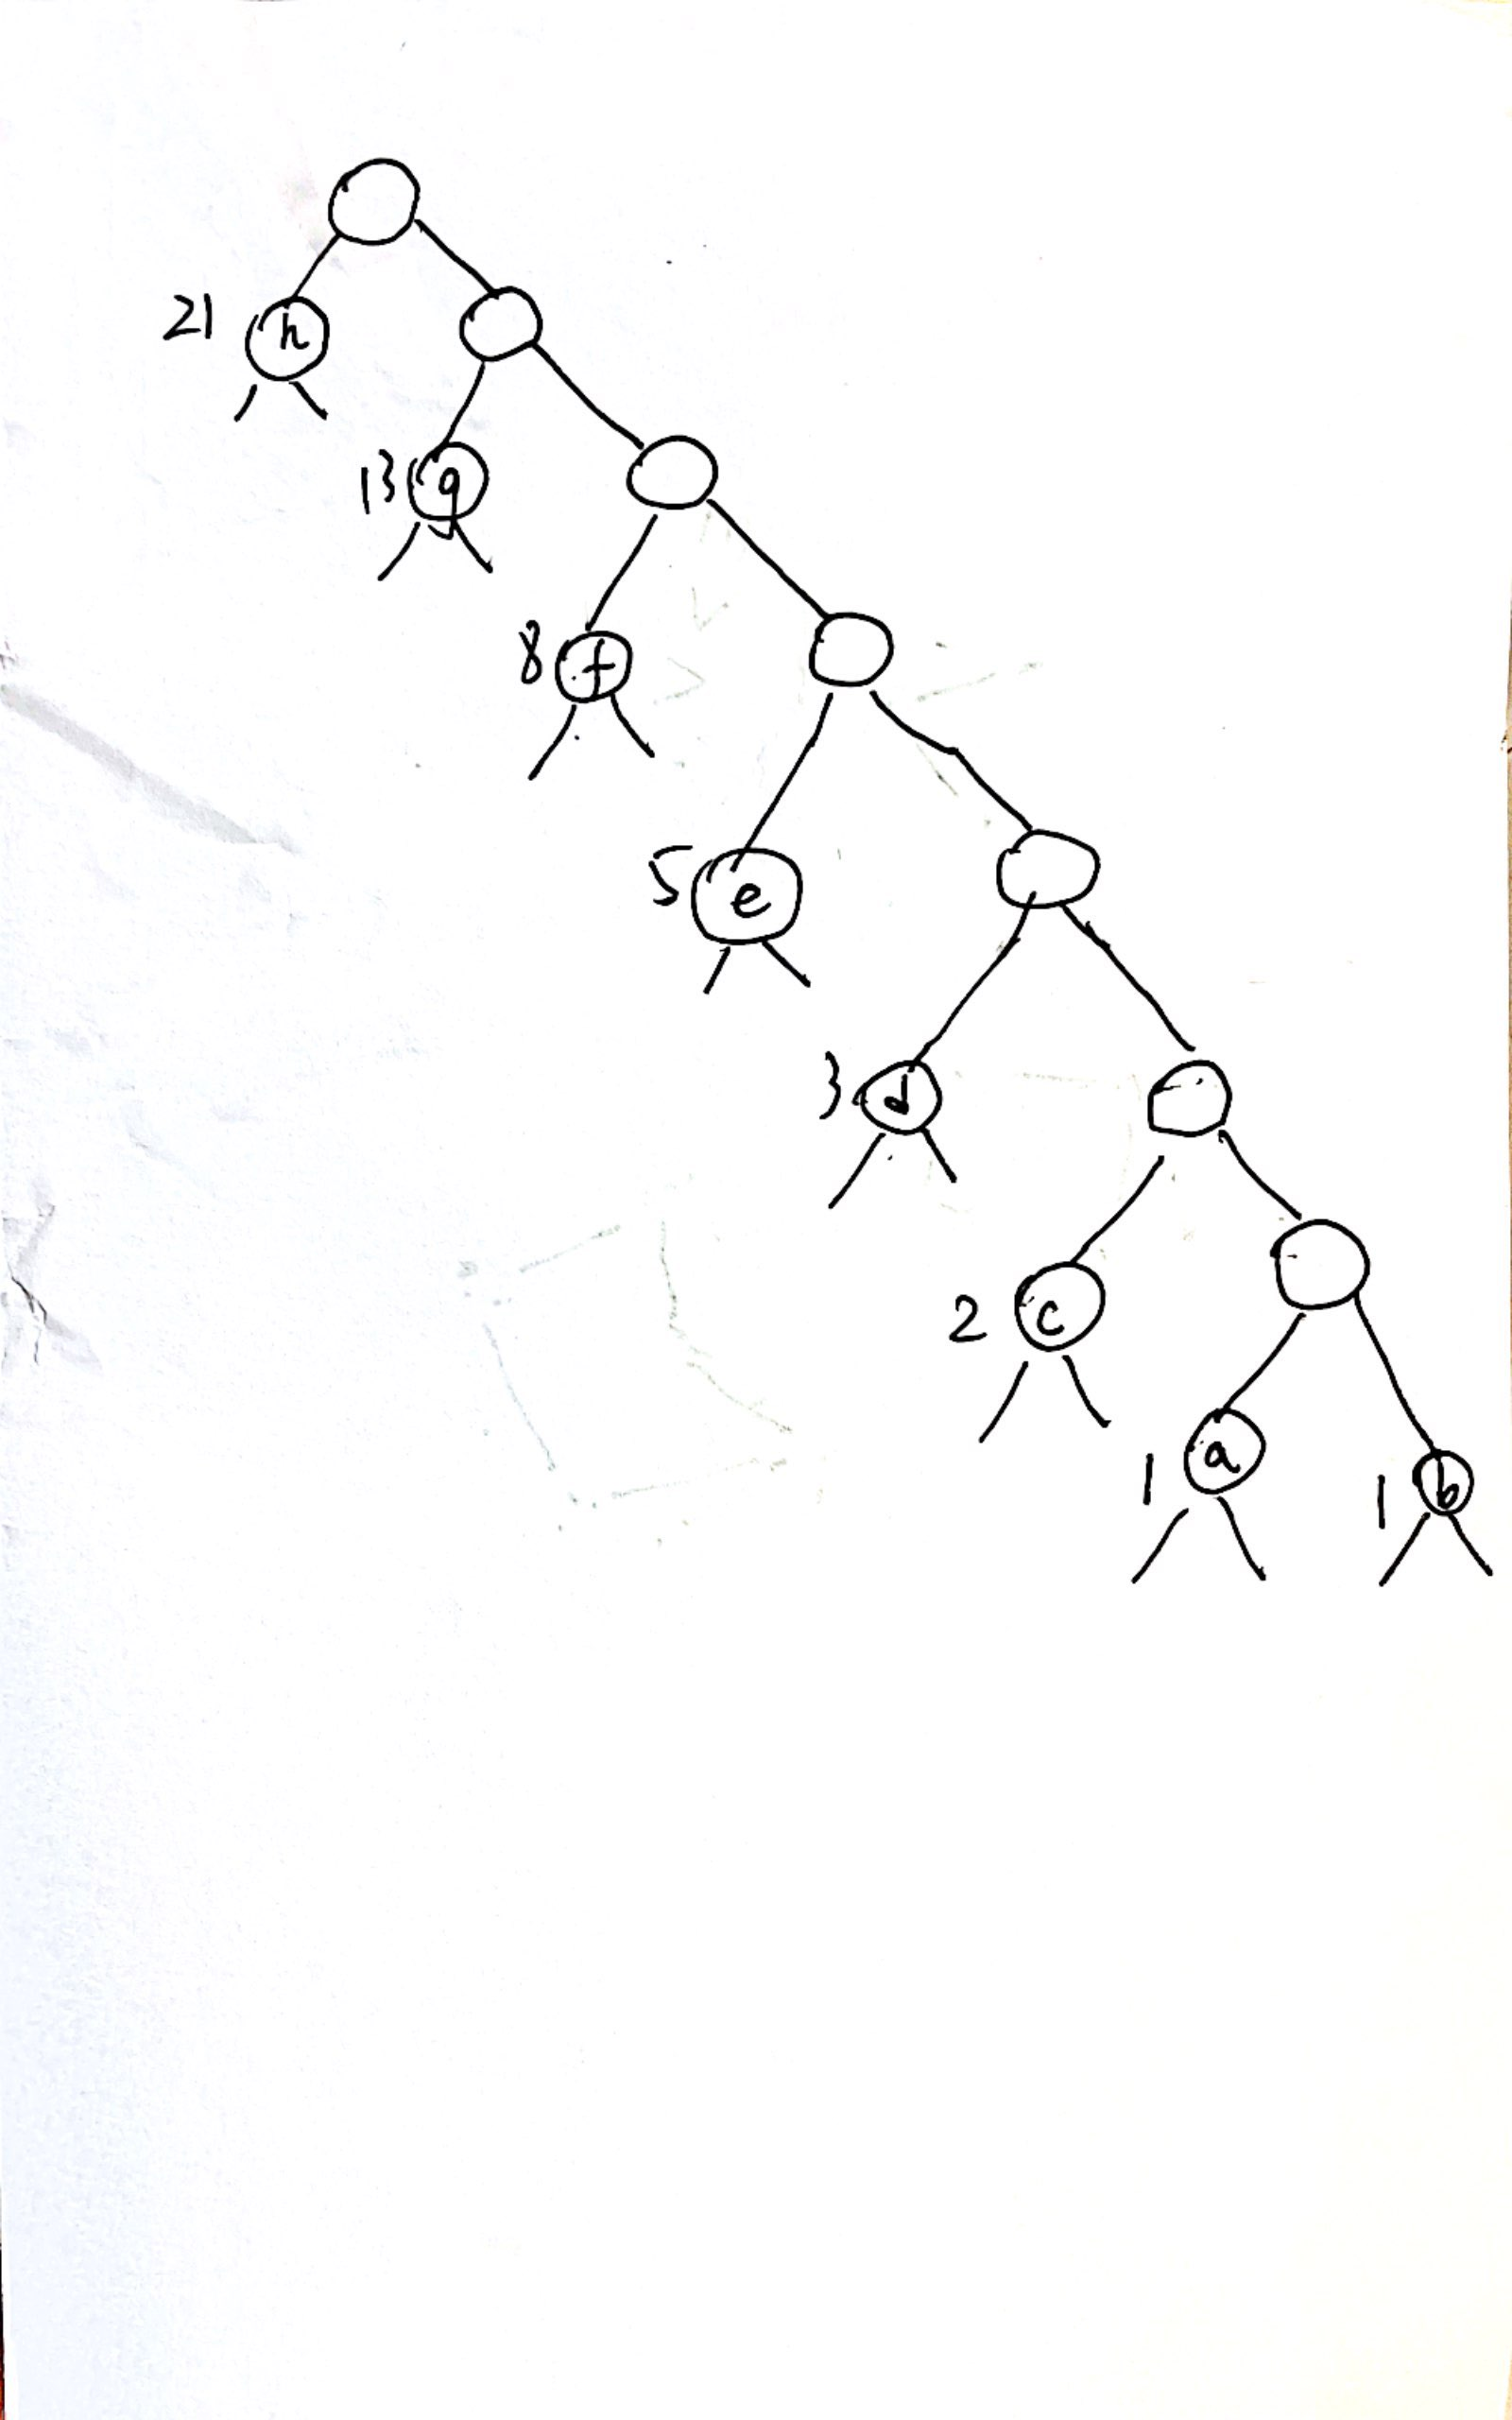
\includegraphics[width=0.5\textwidth]{Huffman_code_result.jpg}
\end{figure}

\newpage
\subsection{Question 8(ii)}
When $n >= 4$, 
\begin{center}
\begin{tabular}{ c c c }
 i-th char & freq & encoding \\ 
 \hline
 $i = 1$ & $F_i$ & $\sum_{k=1}^{n-2} 10^k$ \\   
 $i = 2$ & $F_i$ & $\sum_{k=0}^{n-2} 10^k$ \\  
 $3 \leq i \leq n-1$ & $F_i$ & $\sum_{k=1}^{n-i} 10^k$ \\  
 $i = n$ & $F_i$ & $0$ \\  
\end{tabular}
\end{center}

~\newline\noindent
When $n = 3$, 
\begin{center}
\begin{tabular}{ c c c }
 i-th char & freq & encoding \\ 
 \hline
 $i = 1$ & $F_i$ & $10$ \\   
 $i = 2$ & $F_i$ & $11$ \\  
 $i = 3$ & $F_i$ & $0$ \\  
\end{tabular}
\end{center}

~\newline\noindent
When $n = 2$, 
\begin{center}
\begin{tabular}{ c c c }
 i-th char & freq & encoding \\ 
 \hline
 $i = 1$ & $F_i$ & $0$ \\   
 $i = 2$ & $F_i$ & $1$ \\   
\end{tabular}
\end{center}

\end{document}






